\section{Case Study}

We have used the Object Algebras framework in the implementation of a simple DSL for Questionnaires, called QL~\cite{GPCE}.
A questionnaire is rendered as an interactive form where, depending on user actions, new questions may appear, or values may be computed. 
QL programs consist of lists of labeled, typed questions.
Questions can be answerable, meaning the user has to enter some data, or computed.
In the latter case the question is defined by an expression.
A conditional if-then-else construct allows questions to visually appear only when a certain condition is true. 

To illustrate the utility of \name we have implemented a number of queries and transformations in the context of QL. The queries extract derived information from a QL program, such as the set of used variables, the data and control dependencies between questions and the type environment.
The transformations include two transformations of language extensions to the base language.
The first realizes a simple desugaring of ``unless(c){...}'' to ``if(not(c)){...}''.
The second desugaring statically unfolds a constant bound loop construct (``repeat (i){...}'') and renames variables accordingly.
Finally, we have implemented a simple rename variable operation, and a normalizer which flattens nested conditionals to sequences.  

Table~\ref{TBL:qlresults} shows the number of cases that had to be overridden to implement each particular operation. The top row shows the number of  constructs for each sort in QL (Exp, Stmt, and Form, respectively).
As can be seen, none of the operations required implementing all cases.
For this set of queries and transformations, almost no expression cases needed to be overridden, except the ``Var'' case in collect variables, rename variable and desugar ``repeat''\footnote{Note, however, that the dependency extraction queries reuse the collect variables query on expressions.}.
The cases required for desugaring include the case of the language extension, which is not counted in the total in the top row. 

\begin{table}[t]
  \centering
  \begin{tabular}{l|c|c|c}
    Operation            & Exp (18) & Stmt (5) & Form (1) \\\hline
    Collect variables    & 1              &                &               \\
    Data dependencies    &                & 3               & 1             \\
    Control dependencies &                & 4              & 1             \\
    Type environment     &                & 2              &               \\\hline
    Rename variable      & 1              & 2              &               \\
    Inline conditions    &                & 4              &               \\
    Desugar ``unless''   &                & 1              &               \\
    Desugar ``repeat''   & 1              & 3              &               \\
  \end{tabular}
  \caption{Number of overriden cases per query and transformation in
    the context of the QL implementation\label{TBL:qlresults}}
\end{table}


\subsection{Extending queries and transformations}

Instead of desugaring language extensions to the base language it is also possible to treat them as first-class constructs and retroactively extend existing queries and transformations.
The framework permits to use  Java interface extension to achieve this in a fully type safe way.
Figure~\ref{inline_conds_unless} and Fig.~\ref{controldeps_unless} show the extension of the inline conditions transformation and control dependencies query when extending QL with ``unless''.

\begin{figure}[tb]
\lstinputlisting[linerange=9-16]{../QL/src/_syb/trafo/InlineConditionsUnless.java} % APPLY:linerange=INLINECONDS_UNLESS
\vspace{-.1in}
\caption{Extending the inline-conditions transformation to deal with ``unless''}
\label{inline_conds_unless}
\end{figure}

\begin{figure}[tb]
\lstinputlisting[linerange=10-18]{../QL/src/_syb/query/ControlDepGraphUnless.java} % APPLY:linerange=CONTROLDEPS_UNLESS
\vspace{-.1in}
\caption{Extending the control-dependencies query to deal with ``unless''}
\label{controldeps_unless}
\end{figure}

Inlining of conditions across ``unless'' statements (Fig.~\ref{inline_conds_unless}) is analogous to the implementation for ``if''.
It involves creating a conjunction of the input (\lstinline{guard}) and the negated condition and then passing it down the body of ``unless''. The result is the inlined version of the body.
The extension of the control dependencies (Fig.~\ref{controldeps_unless}) query simply delegates to the implementation of ``if'' (\lstinline{iff}). 

\subsection{\name performance vs Vanilla ASTs}

\begin{figure}[t]
  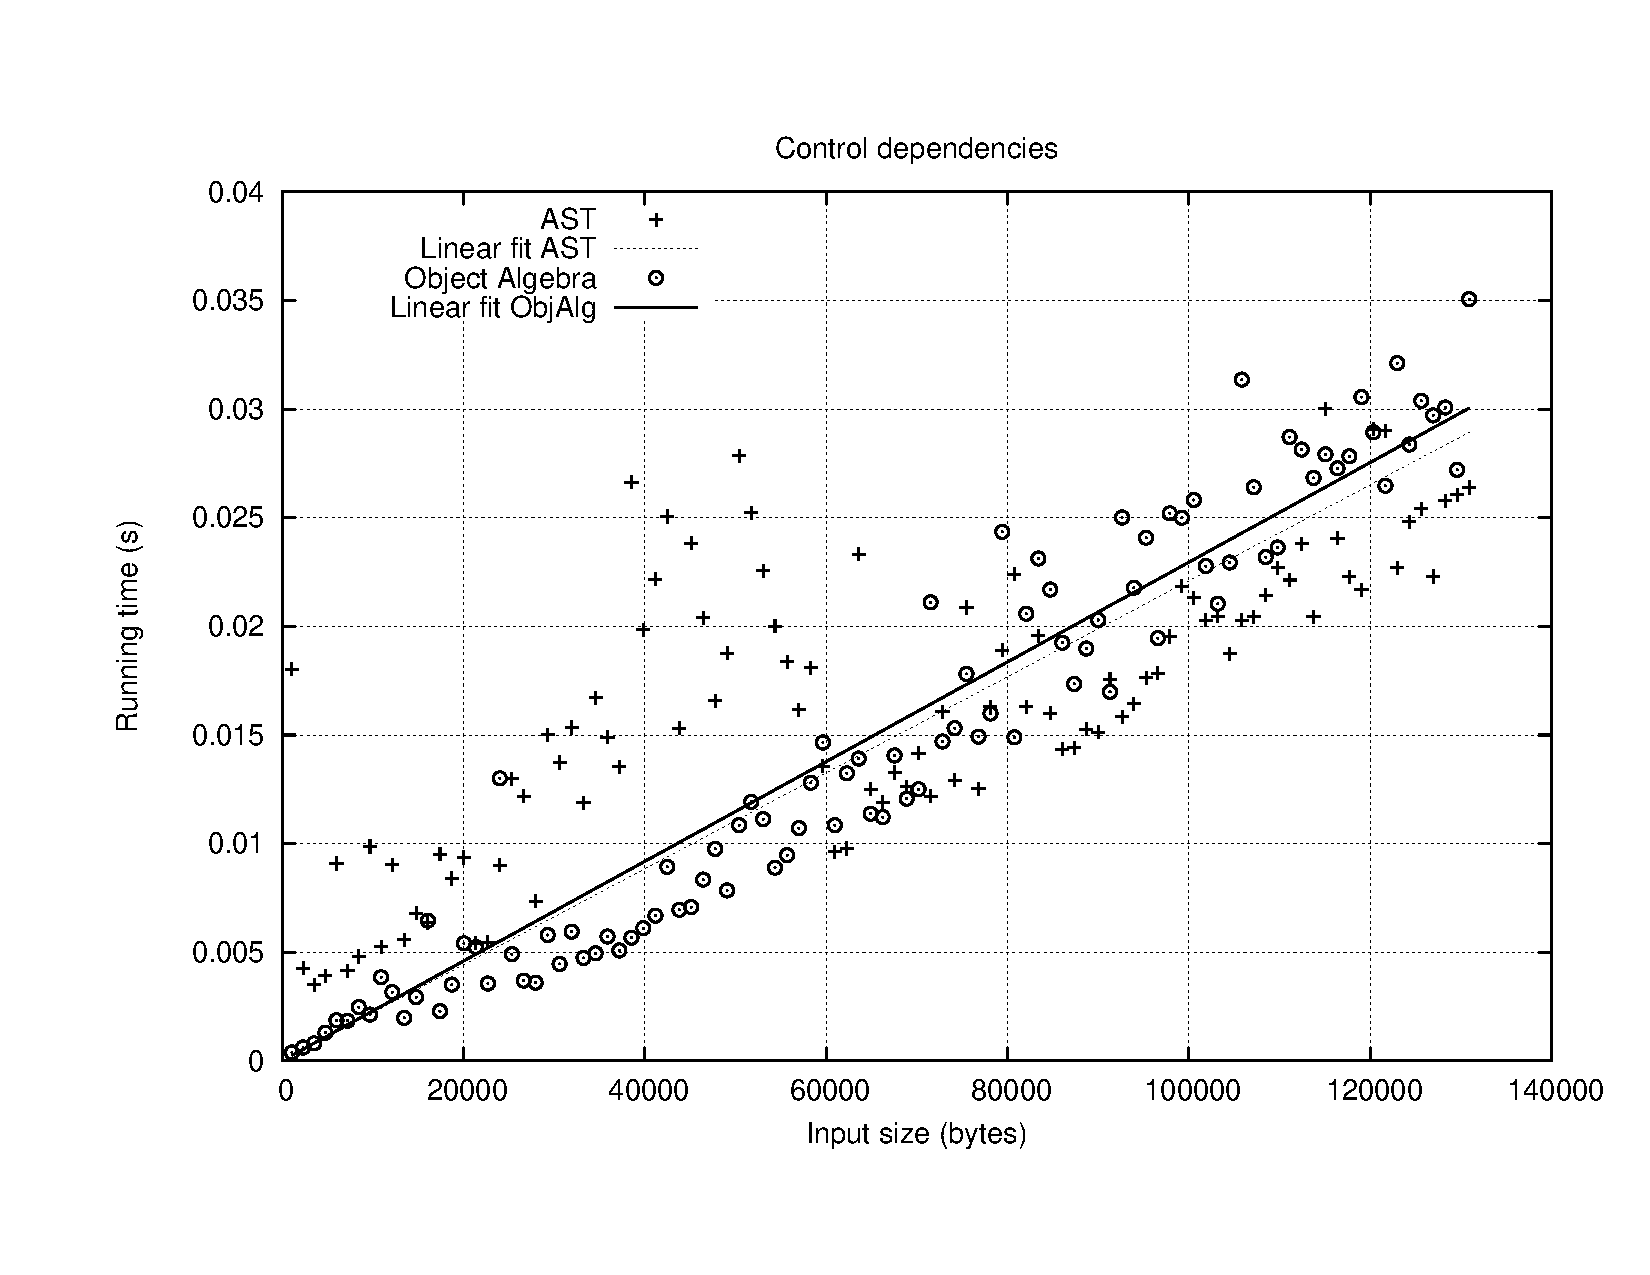
\includegraphics[width=0.49\textwidth]{plots/controldeps}
  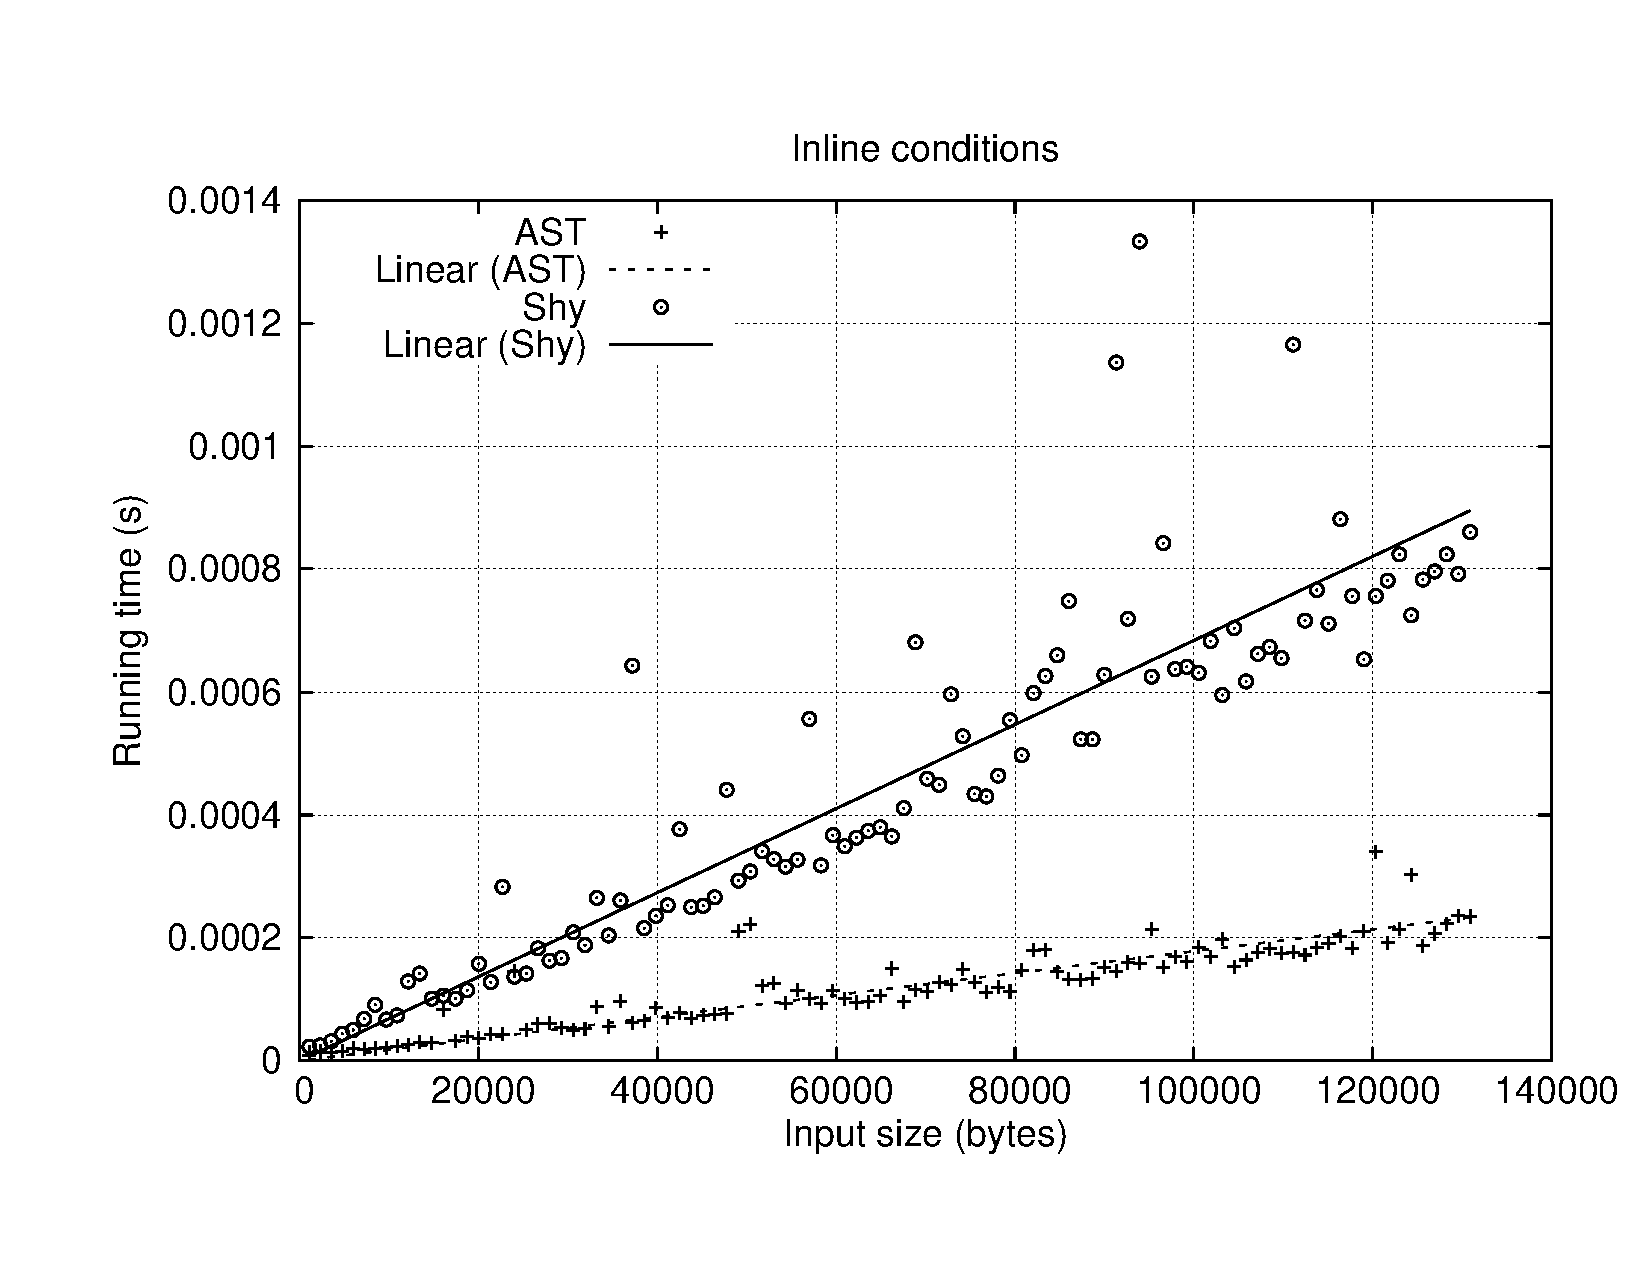
\includegraphics[width=0.49\textwidth]{plots/inline}
  \caption{Performance comparison of control dependencies query (left) and inline conditions transformation (right) implemented using normal ASTs vs using the \name framework\label{FIG:performance}}
\end{figure}

We compared the performance characteristics of the operations implemented using \name with respect to vanilla implementations based on ordinary AST classes.
The operations were executed on progressively larger QL programs (up to 1.4Mb).
In the vanilla implementation, the program was parsed into an AST structure, and then the operation was invoked and measured.
In the case of the \name queries, constructing the ``AST'' corresponds to executing the query, so we measured that.
For context-dependent transformation, however, building the ``AST'' corresponds to constructing the function to execute the transformation, hence we only measured the execution of invoking this function. 
To make the comparison as fair as possible, the query implementations use the same monoid structures as in \name.

The comparison of the control dependencies query is shown on the left of Fig.~\ref{FIG:performance}.
The plot shows that the performance is quite comparable.
On average, the \name implementation of the query seems a little slower.
This is probably caused by the extensive use of interfaces in the \name framework, whereas the AST-based implementation only uses abstract and concrete classes \tijs{NEED REFERENCE!!!!, but see: \url{http://stackoverflow.com/questions/6839943/why-are-interface-method-invocations-slower-than-concrete-invocations}}.

For transformations the performance difference is slightly more severe.
The right of Fig.~\ref{FIG:performance} shows the performance comparison of the inline conditions transformation. 
The greate difference can probably be explained by the fact that creating a new structure in a \name transformation involves dynamically dispatched method calls instead of statically bound constructor calls. 




